\section{Results}
    \begin{frame}
    \frametitle{Outline}
    \begin{columns}[T]
        \begin{column}{.45\textwidth}
            \tableofcontents[sections=1-3,currentsection]
        \end{column}
        \begin{column}{.45\textwidth}
            \tableofcontents[sections=4-5,currentsection]
        \end{column}
    \end{columns}
    \end{frame}

\subsection{Transitory Regime}
\begin{frame}{\subsecname}
    
\begin{figure} [H]  
	\centering
	\subfloat
	{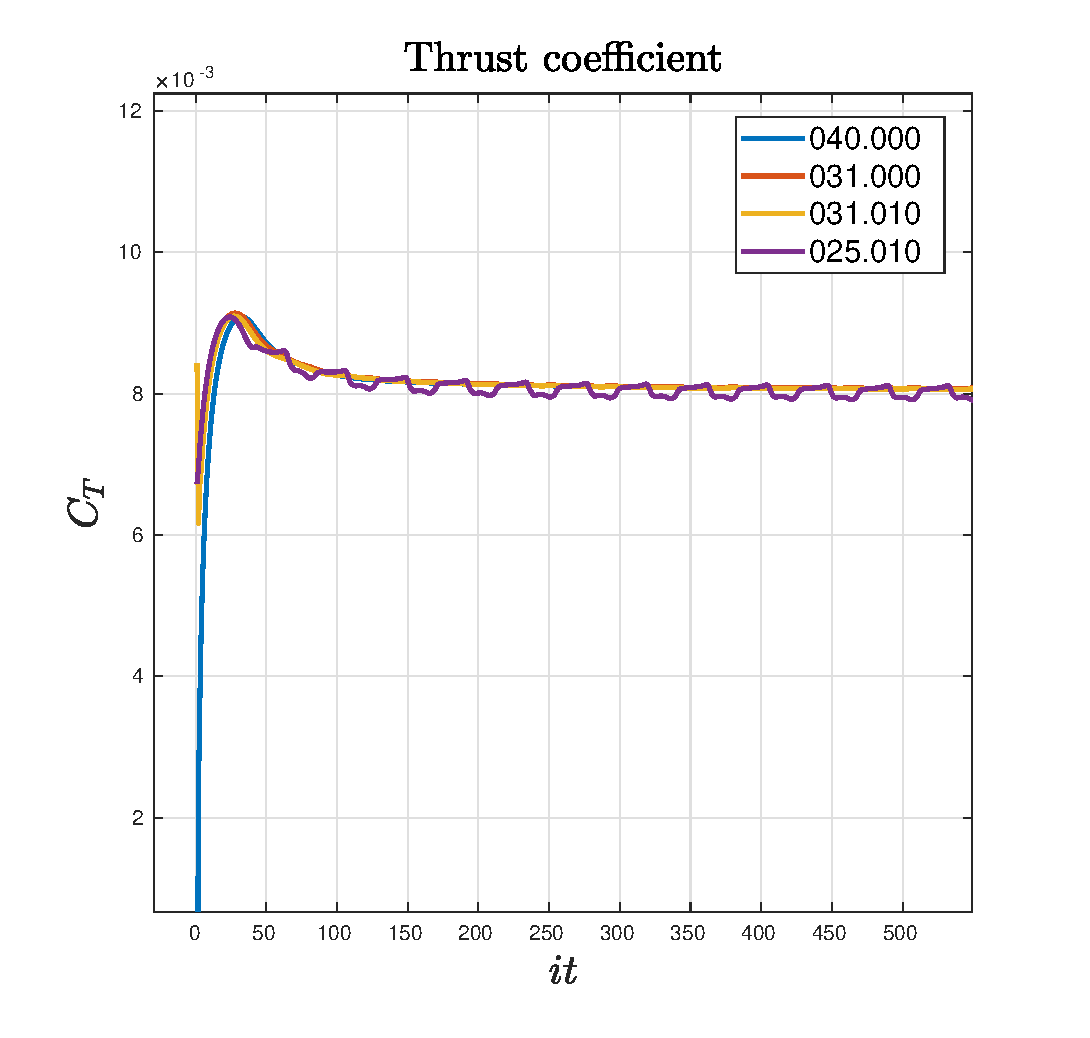
\includegraphics[scale=0.30]{Photos/Ct_iter.eps}}
  \quad
	\subfloat
	{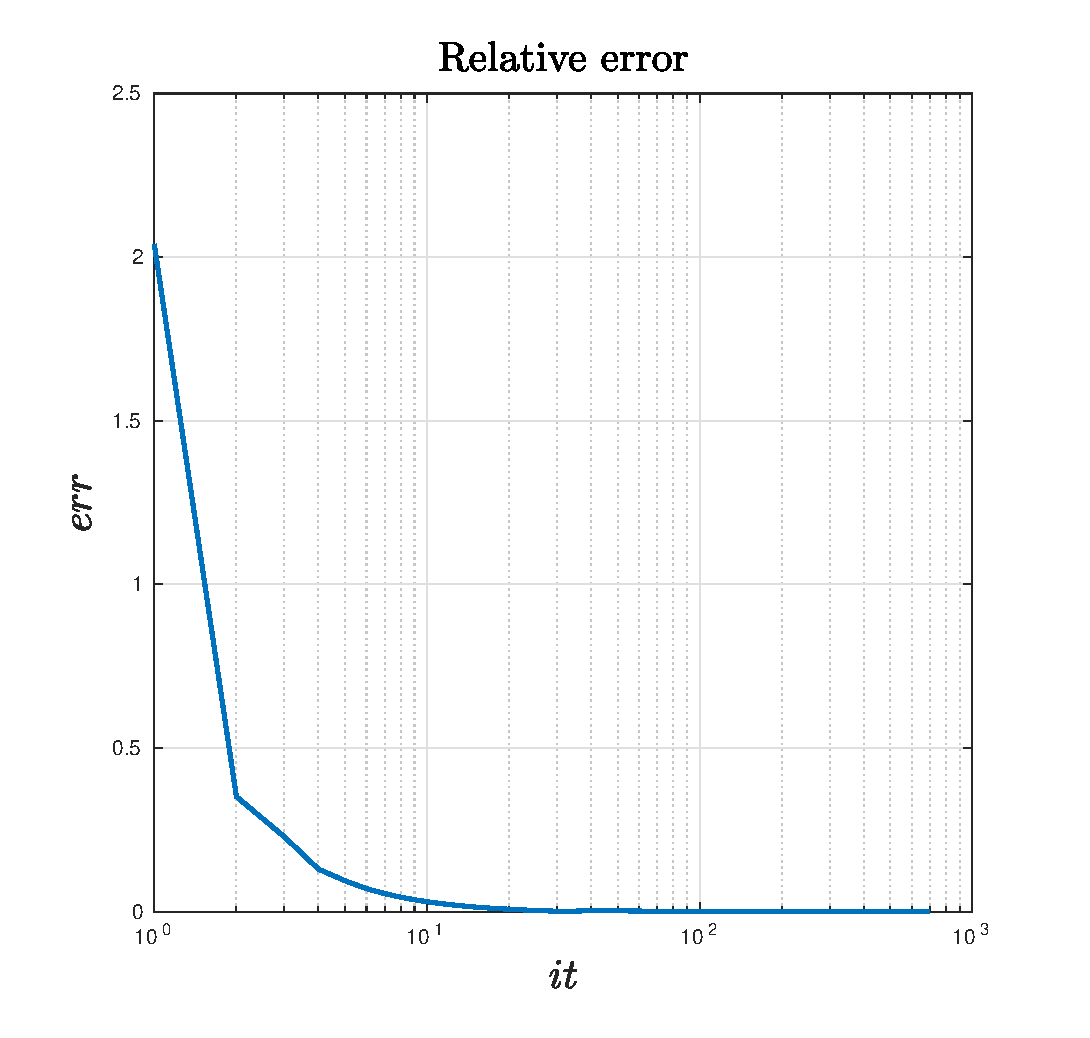
\includegraphics[scale=0.30]{Photos/err_iter.eps}
  }
\end{figure} 
\begin{center}
\vspace{-0.4cm}
 $c_T = \frac{T}{\rho n^2 D^4}$ \hspace{4cm} $err = \frac{\abs{c_T^{i+1}- c_T^{i}}}{c_T^{i+1}}$
 \newline
 \newline
    1 rev = 128 iter $\xrightarrow{}$ Stationary regime after 3 revs = 384 iter
\end{center}

\end{frame}

\subsection{SPL: Two rotors }
\begin{frame}{\subsecname}

\begin{figure} [H]  
	\centering
	\subfloat
	{\includegraphics[scale=0.35]{Photos/spl_2rot_040000_031000.eps}}
  %\quad
	\subfloat
	{\includegraphics[scale=0.35]{Photos/spl_2rot_031000_031010.eps}
  }
\end{figure} 
\end{frame}

\begin{frame}{\subsecname}
\begin{figure} [H]  
	\centering
	\subfloat
	{\includegraphics[scale=0.35]{Photos/spl_2rot_031010_025010.eps}}
  %\quad
	\subfloat
	{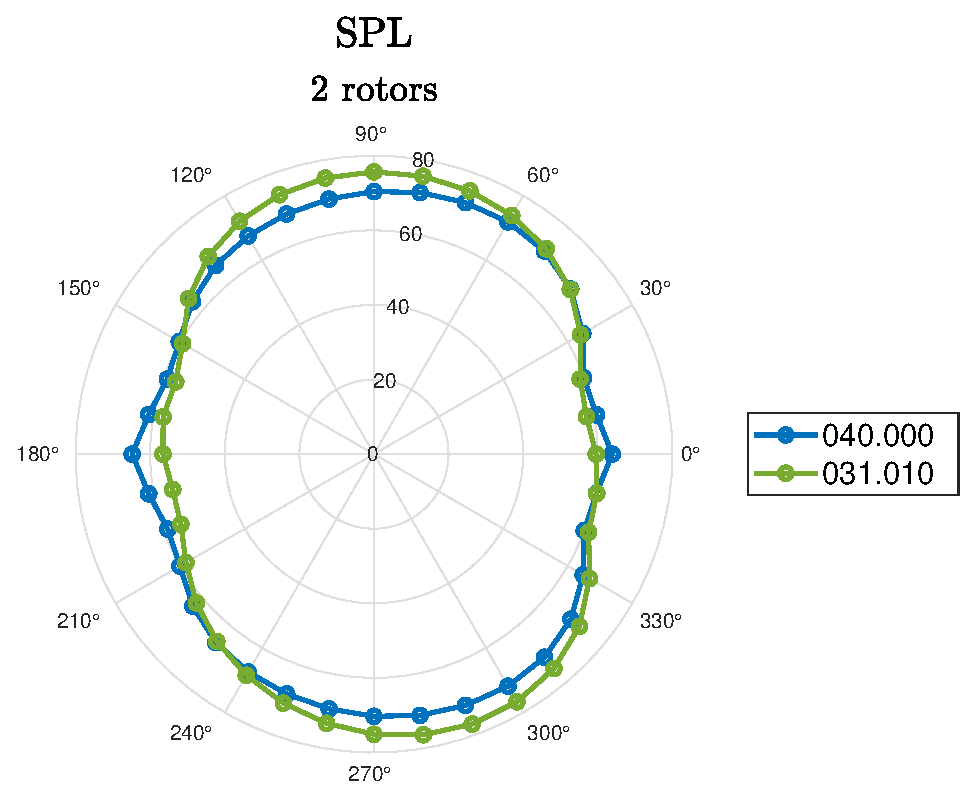
\includegraphics[scale=0.35]{Photos/spl_2rot_040000_031010.eps}
  }
\end{figure} 

\end{frame}

 \subsection{Pressure Fluctuation}
\begin{frame}{\subsecname}
    \begin{figure} [H]  
	\centering
	\subfloat [$\Delta t$ = 9.09x10$^{-4}$ s]
	{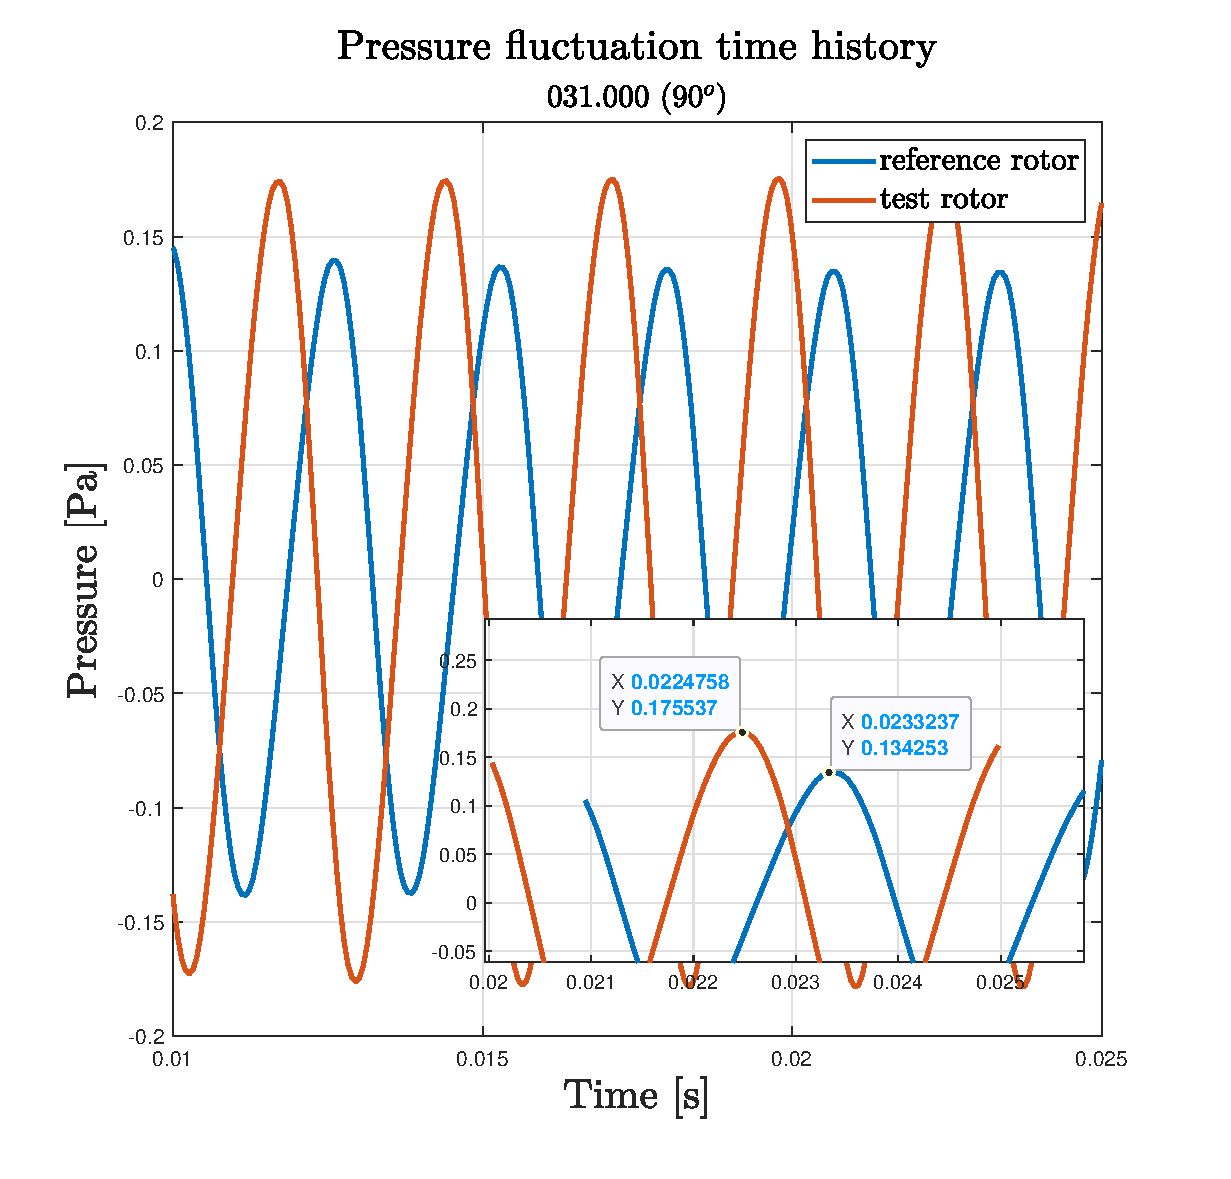
\includegraphics[scale=0.27]{Photos/phase_shift_031000.eps}}
  \quad
	\subfloat [$\Delta t$ = 1.12x10$^{-3}$ s]
	{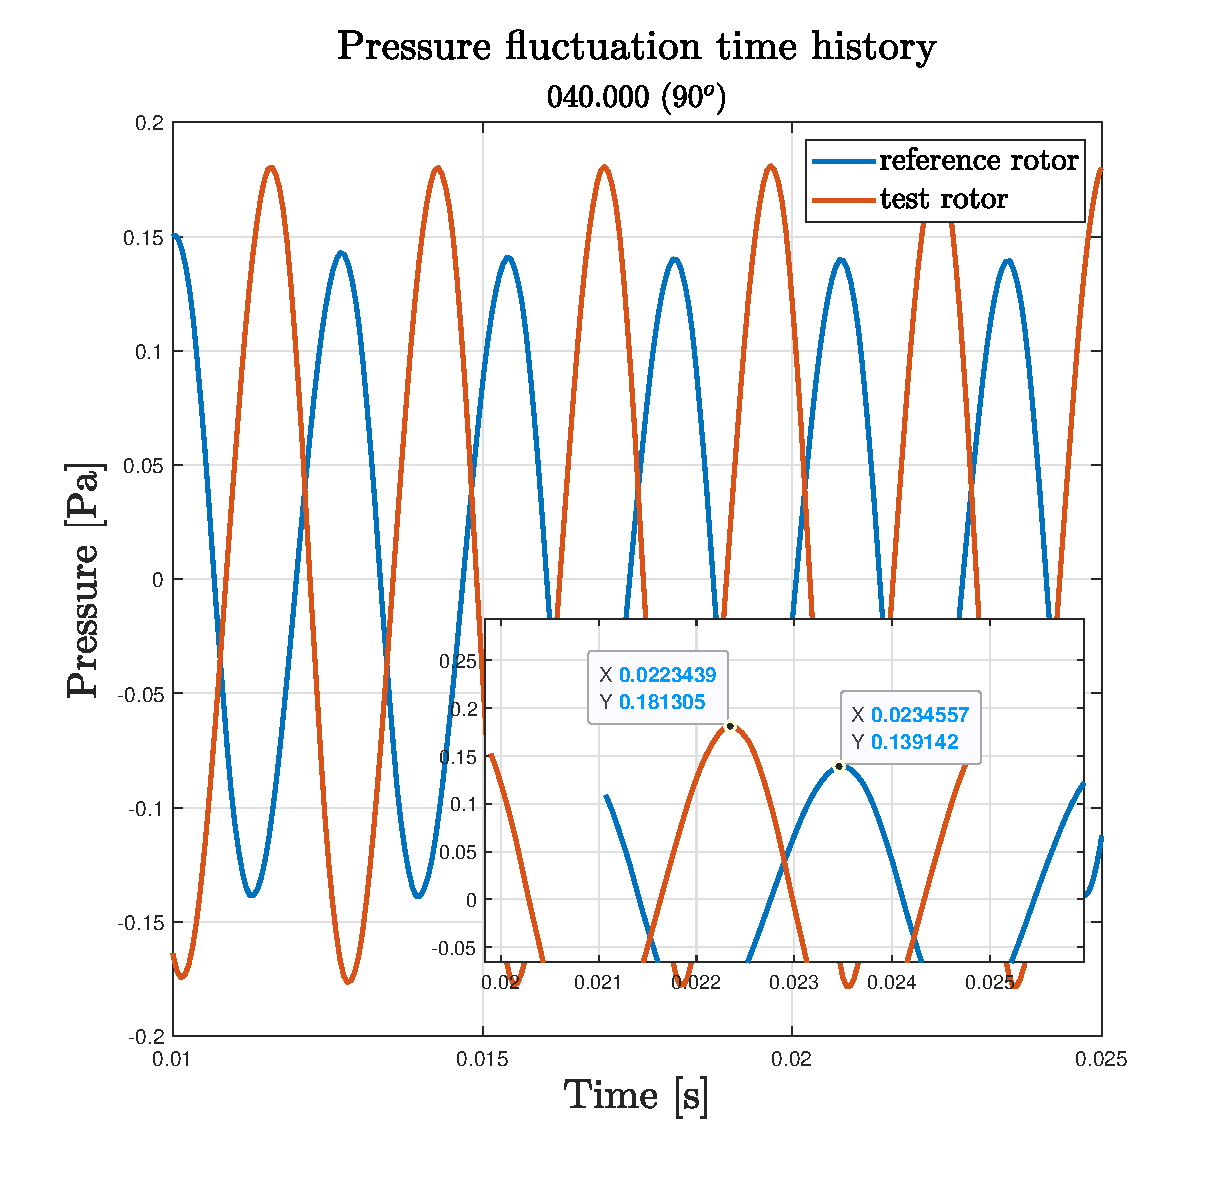
\includegraphics[scale=0.27]{Photos/phase_shift_040000.eps}
  }
\end{figure} 
    
\end{frame}

\subsection{PSD}
\begin{frame}{\subsecname}
    \begin{figure} [H]  
	\centering
	\subfloat
	{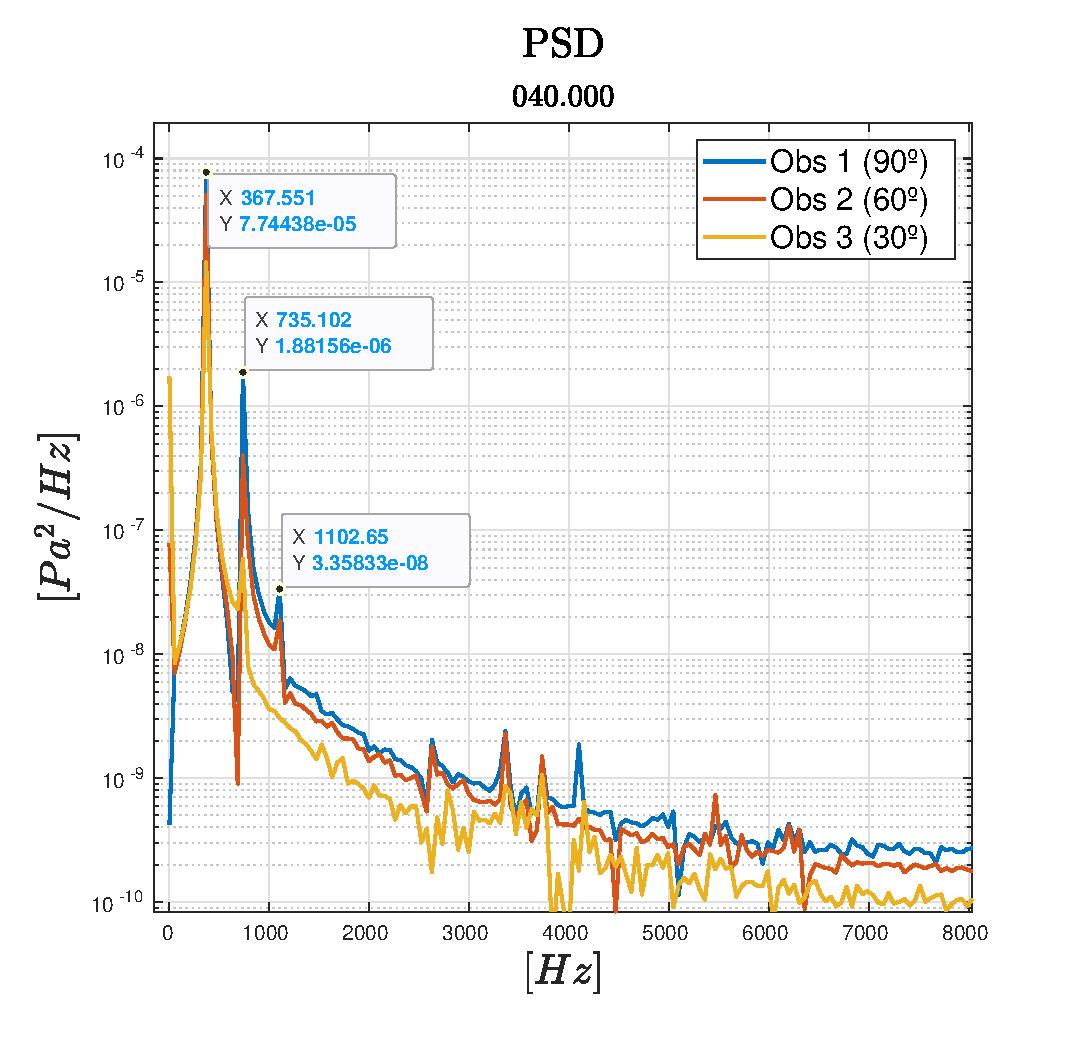
\includegraphics[scale=0.305]{Photos/psd_040000.eps}}
  \quad
	\subfloat
	{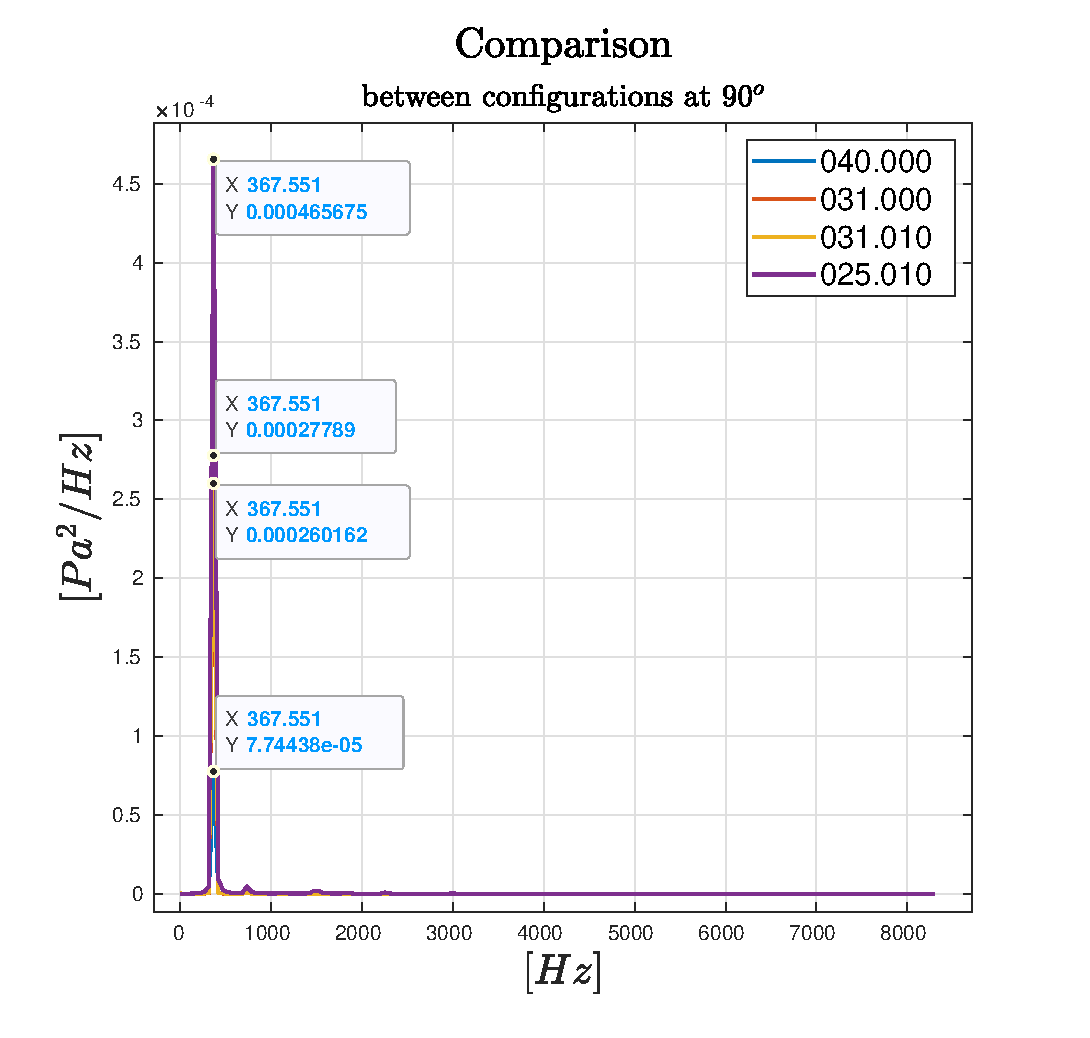
\includegraphics[scale=0.305]{Photos/psd_comparison.eps}
  }
\end{figure}
\begin{center}
    
\resizebox{8cm}{!}{
 \begin{table}[H]
                %\caption*{\textbf{Title of Table (optional)}}
                \centering 
                \begin{tabular}{|c c c |}
                \hline
                \rowcolor{bluePoli!40 } % bluePoli!40 comment this line to remove the color
                  Sampling frequency [$Hz$] & Time Step [$s$] & Signal duration [$s$]\T\B \\
                \hline \hline
                1.6726x10$^4$ & 6.6514x10$^{-5}$ & 0.08514 (10 rev)\T\B  \\
                \hline
                \end{tabular}
    \end{table}}
    \end{center}
\end{frame}



\subsection{SPL: One rotor}
\begin{frame}{\subsecname}
    \begin{figure} [H]  
	\centering
	\subfloat
	{\includegraphics[scale=0.35]{Photos/spl_1rot_040000_single.eps}}
 % \quad
	\subfloat
	{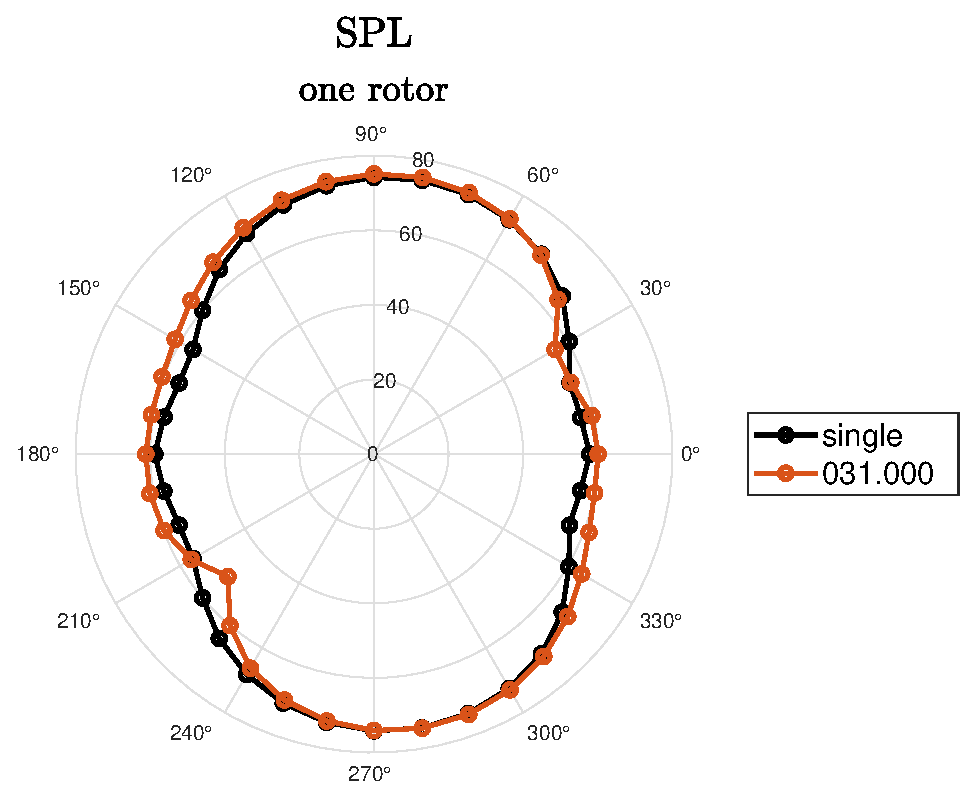
\includegraphics[scale=0.35]{Photos/spl_1rot_031000_single.eps}
  }
\end{figure} 
\end{frame}

\begin{frame}{\subsecname}
    \begin{figure} [H]  
	\centering
	\subfloat
	{\includegraphics[scale=0.35]{Photos/spl_1rot_031010_single.eps}}
 % \quad
	\subfloat
	{\includegraphics[scale=0.35]{Photos/spl_1rot_025010_single.eps}}
\end{figure} 
\end{frame}

\subsection{Tonal Noise: One rotor}
\begin{frame}{\subsecname}
    \begin{figure} [H]  
	\centering
	\subfloat
	{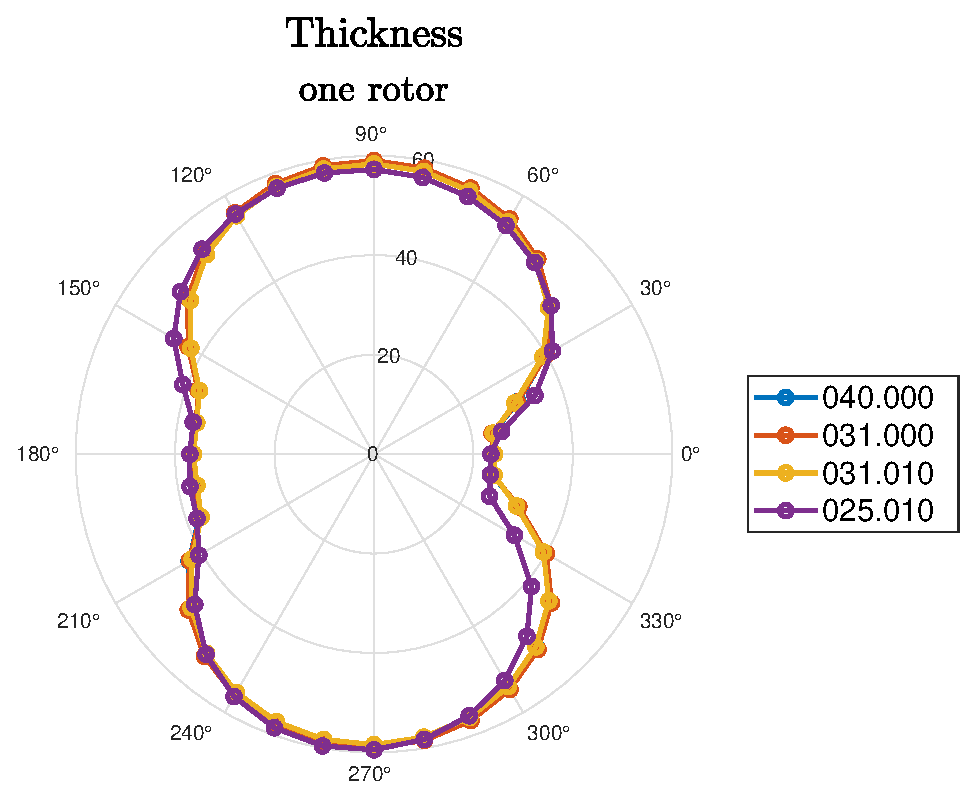
\includegraphics[scale=0.35]{Photos/thickness_comparison.eps}}
  %\quad
	\subfloat
	{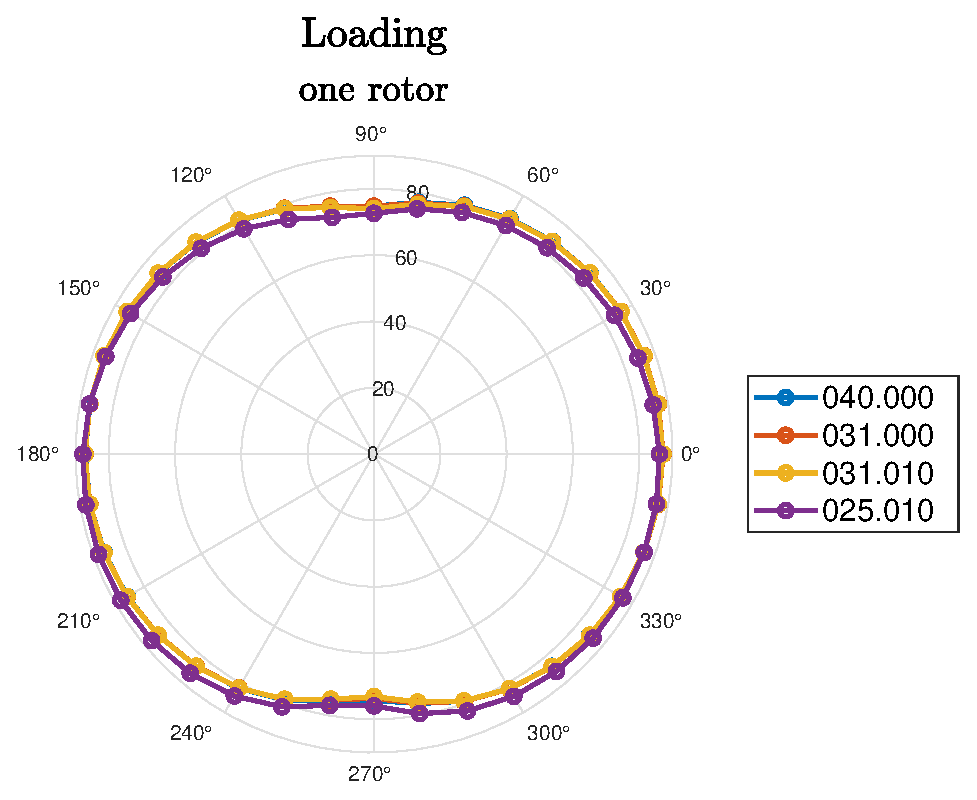
\includegraphics[scale=0.35]{Photos/loading_comparison.eps}
  }
\end{figure} 
\end{frame}

